\chapter{Design of Arabic RAG-Based Agent for Legal and Juridical Data.}
\pagestyle{fancy}\lhead{\textbf \footnotesize\it{Design of Arabic   RAG-Based Agent for Legal data}}
\pagestyle{fancy}\chead{} \pagestyle{fancy}\rhead{}
\pagestyle{fancy}\cfoot{} \pagestyle{fancy}\rfoot{\thepage}
%%%%%%%%%%%%%%%%%%%%%%%%%%%%%%%%%%%%%%%%
\section{Introduction}\label{start4}
The growing demand for intelligent legal assistance has highlighted the need for domain-specific natural language processing NLP systems. This chapter presents the development of a Retrieval-Augmented Generation RAG Agent tailored for Arabic legal texts. The primary goal of this Agent is to answer legal queries accurately by leveraging a combination of dense information retrieval and generative language modeling. By integrating Arabic legal domain knowledge with advanced retrieval techniques and generative models, the Agent delivers explainable, high-quality responses grounded in real case data. This chapter outlines the complete pipeline—from dataset design and model training to evaluation—offering insights into the construction of a practical and robust Arabic legal chatbot.


\section{Dataset Design}
For the development of the Arabic RAG Agent tailored to the legal domain, two purpose-built datasets were created: the Legal Case Dataset and the QA Dataset. These datasets form the foundation of the RAG pipeline, enabling both effective retrieval and accurate answer generation. The Legal Case Dataset consists of actual legal rulings published by the Algerian Supreme Court, while the QA Dataset includes synthetic question-answer pairs generated from those rulings. By combining rule-based techniques with generative modeling, the Agent benefits from both structure and linguistic variability, helping it generalize better during answer generation and evaluation.
\begin{table}[h!]
	\centering
	\captionsetup{justification=centering}
	\renewcommand{\arraystretch}{1.4}
	\begin{tabularx}{\textwidth}{|>{\raggedright\arraybackslash}p{2.5cm}|>{\raggedright\arraybackslash}p{3.1cm}|>{\raggedright\arraybackslash}p{3cm}|>{\raggedright\arraybackslash}p{3.2cm}|>{\raggedright\arraybackslash}X|}
		\hline
		\textbf{Dataset Name} & \textbf{Description} & \textbf{Structure} & \textbf{Use Case} & \textbf{Construction Method} \\
		\hline
		Legal Case Dataset & 104 Arabic legal cases collected from the Algerian Supreme Court journal & Case ID, Title, Keywords, Description & Used for building the retriever index and generating QA pairs & Scraped from the official court journal and manually cleaned, labeled, and structured \\
		\hline
		QA Dataset & 512 question-answer pairs derived from the legal case dataset & Case ID, Question, Answer, Context, Context Tokens & Used for training, generation, and evaluation of the RAG Agent & Constructed using a hybrid approach: rule-based extraction of key legal elements + generative QA using AraGPT2 \\
		\hline
	\end{tabularx}
	\caption{Summary of the datasets used in the Arabic Legal RAG Agent}
\end{table}
Figure~\ref{dataset_creation} illustrates the detailed pipeline used for the creation of both the legal case dataset and the corresponding question-answer (QA) dataset. The process begins with web scraping from official Algerian court sources, followed by data cleaning and normalization. Subsequently, the normalized legal data is utilized to generate QA pairs through both , resulting in a structured dataset suitable for Arabic legal question answering tasks.
\begin{figure}[h]
	\centering
	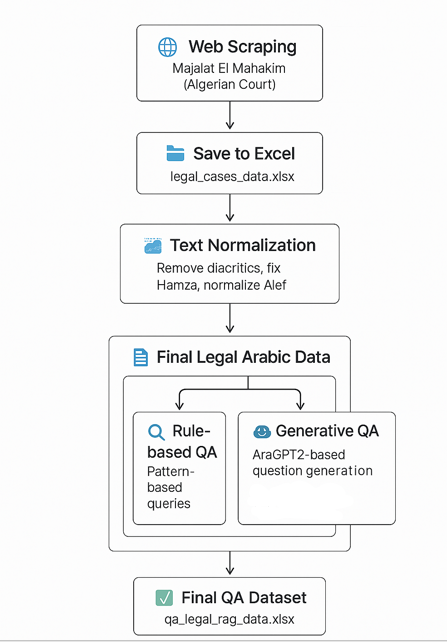
\includegraphics[width=0.5\linewidth]{Figures/dataC.png}
	\caption{The detailed pipeline used for the creation of both the legal case dataset and the  question-answer QA}
	\label{dataset_creation}
	
\end{figure}

\newpage
\section{Agent Architecture Overview}
To build an Arabic legal assistant capable of answering questions about legal cases, we adopted an agentic architecture based on  RAG. The Agent is composed of modular components that work together to understand user questions, retrieve relevant legal content, and generate informative responses. It is designed to handle complex legal texts and support both general legal queries and specific requests, such as extracting particular legal articles Figure~\ref{agentic_architecture} illustrates Agent Architecture Overview.
\begin{figure}[h]
	\centering
	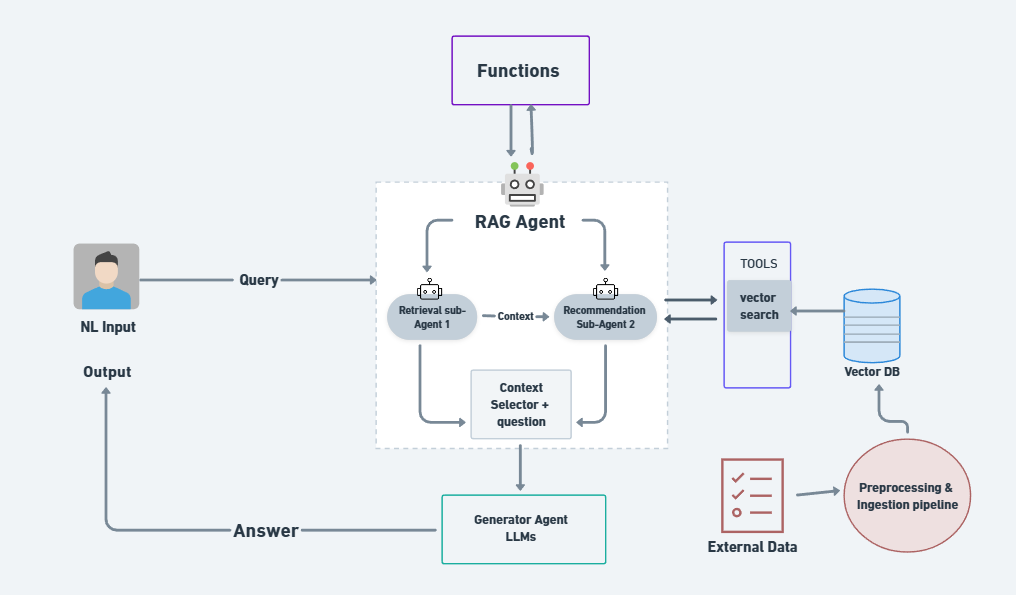
\includegraphics[width=0.9\linewidth]{Figures/agentarchi.png}
	\caption{Architecture of the Arabic RAG-Based Agent for Legal Data. The Agent takes Arabic natural-language questions as input and returns answers grounded in real legal case context. It integrates preprocessing, semantic retrieval, and generation agent. }
	
	\label{agentic_architecture}
	
\end{figure}

\subsection{Input/Output}

The agent \textbf{receives natural-language arabic questions as input}. These questions may range from general inquiries about a legal case to specific prompts requesting certain materials, such as legal articles. As output, the Agent\textbf{ returns either detailed answers grounded in real legal case context or a filtered subset of legal references} (e.g., materials/articles), depending on the nature of the user request.

\subsection{Preprocessing and Ingestion Phase}
Before retrieval and generation, legal documents go through a data ingestion pipeline. This includes cleaning and normalizing raw text, followed by semantic chunking to ensure each unit of information is appropriately sized. These chunks are then embedded and indexed into a vector database to enable efficient semantic retrieval during runtime. This phase ensures the quality, structure, and retrievability of legal content.

\subsection{Retriever Sub-Agent }
The retriever identifies the most relevant pieces of legal content based on the user’s query. It searches through the vectorized representation of the case database to return a ranked list of the most semantically similar chunks. This retrieval process ensures that the agent has access to high-quality and contextually relevant legal information.

\subsection{Recommendation Sub-Agent}
If the user's request targets specific legal materials (e.g., legal articles mentioned within a case), a recommendation sub-agent is triggered. This agent scans the previously retrieved content to identify and extract only the relevant sections that match patterns typically associated with legal article references. This sub-agent demonstrates intra-agent communication, as it relies on outputs from the main retriever while adding a specialized capability.
\subsection{Context Selector: Token-Aware Filtering}
From the retrieved candidates, the agent selects the most relevant chunks that fit within the system’s input constraints. This filtering ensures that the generator receives coherent, non-redundant, and contextually rich text to support accurate response generation.
\subsection{Functions and Tools}
In addition to the core RAG-based workflow, the architecture integrates a flexible function-calling and tool-use mechanism. This enables the agent to interact with external tools—such as file analyzers, legal databases. These tools are invoked dynamically based on the user query, and the outputs are fed back into the RAG Agent to support more grounded, context-aware answers.


\subsection{Generator: Answer Formulation Component}
Using the selected context, the generator produces a coherent and legally grounded answer in Arabic. The generation process is context-aware, allowing it to reflect the nuances of legal terminology and adapt the output style depending on the user’s request.

\subsection{Agent Design}
The core Agent functions as a domain-specific legal agent that uses Retrieval-Augmented Generation to assist users with legal case questions. It is capable of:

\begin{itemize}
	\item Understanding natural Arabic legal questions, including complex legal terminology.
	\item Retrieving relevant information from legal case texts using semantic search.
	\item Generating answers grounded in real legal content.
	\item Recommending specific legal materials when requested by the user.
\end{itemize}

Rather than relying on predefined responses, the agent dynamically retrieves and composes answers using the most relevant and up-to-date case context. It can be used by legal professionals, students, or institutions to enhance legal understanding and streamline research across a wide range of case types.
\section{Training the Agent}
To empower the Arabic RAG-Based Agent with accurate and context-aware responses, we trained both its retriever and generator components on a curated Arabic legal QA dataset. This training phase focused on optimizing the agent’s ability to understand user questions, retrieve the most relevant legal context, and generate coherent and grounded answers.
\begin{figure}[h]
	\centering
	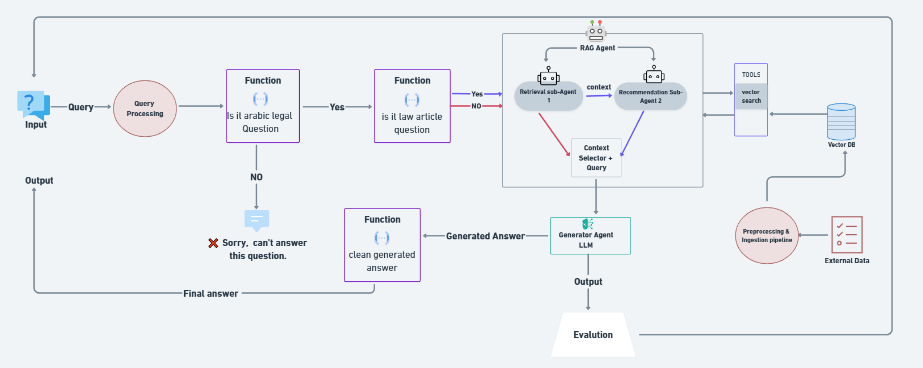
\includegraphics[width=0.8\linewidth]{Figures/trainingagent.png}
\caption{An overview of the training pipeline for the RAG agent }
	
	\label{agentic_trining}
	
\end{figure}


\subsection{Training the Retriever}
The retriever is responsible for identifying and retrieving the most relevant legal context for a given user query. This component can be trained or configured through several key phases that focus on data preprocessing, semantic embedding, and efficient indexing. Below, we outline a generalizable framework for training a dense retriever in Arabic legal RAG Agent.

\begin{itemize}
	\item \textbf{Text Normalization Pipeline:}
	A preprocessing stage is essential to clean and standardize Arabic legal texts. This may involve:
	\begin{itemize}
		\item Removing diacritics to minimize lexical variations.
		\item Normalizing common character variants (e.g., Alef, Taa Marbouta).
		\item Standardizing punctuation symbols and quotation marks.
		\item Eliminating excess whitespace and formatting inconsistencies.
	\end{itemize}
	
	\item \textbf{Document Chunking Strategy:}
	Legal documents are often lengthy and need to be divided into smaller, semantically coherent chunks. Common techniques include:
	\begin{itemize}
		\item Using recursive text splitters with a fixed token size (e.g., 300 or 500 tokens).
		\item Applying hierarchical splitting rules (paragraphs, then sentences, then phrases).
		\item Preserving key metadata like title, keywords, or article number.
		\item Leveraging tokenizer-based length calculation to ensure chunk boundaries match model requirements.
	\end{itemize}
	
	\item \textbf{Dense Retrieval Architecture:}
	Semantic search typically relies on encoding both documents and queries into dense vector representations using transformer-based models. Common considerations include:
	\begin{itemize}
		\item Choosing a pre-trained multilingual or Arabic-specific embedding model.
		\item Applying mean pooling or CLS token extraction to produce sentence-level embeddings.
		\item Normalizing embeddings (e.g., via L2 normalization) to improve similarity computation.
		\item Using batch processing for faster embedding generation on GPU or CPU.
	\end{itemize}
	
	\item \textbf{Indexing Framework:}
	To enable efficient similarity search, embedding vectors can be stored in a specialized vector database or indexing engine. Some popular practices include:
	\begin{itemize}
		\item Using FAISS or other vector stores to build inner-product or approximate nearest neighbor indices.
		\item Associating each embedding with its original text and metadata.
		\item Tracking chunk-document mappings for traceability during retrieval.
	\end{itemize}
	
	\item \textbf{Query Processing:}
	The user question must be preprocessed and embedded in the same way as documents. Key steps may involve:
	\begin{itemize}
		\item Prefixing or formatting the query to match model expectations.
		\item Applying the same normalization steps used during indexing.
		\item Calculating similarity scores (e.g., cosine similarity) between query and document vectors.
		\item Returning the top-k matching chunks with associated document IDs or metadata.
	\end{itemize}
	
	\item \textbf{Evaluation Dataset:}
	Evaluating retrieval quality typically involves a labeled dataset containing questions, gold answers, and corresponding contexts. This can be used to measure:
	\begin{itemize}
		\item Retrieval accuracy metrics such as :
		\begin{enumerate}
			\item  Recall@K measures the proportion of queries where the correct case appears in the top-K results,
			\item  MRR (Mean Reciprocal Rank) emphasizes the position of the first correct result through reciprocal weighting. 
			\item Hit@K provides a binary success indicator for each query. 
		\end{enumerate}
		\item Relevance of retrieved contexts with respect to the ground-truth legal passages.
		\item The impact of retrieval quality on downstream answer generation.
	\end{itemize}
\end{itemize}
\subsection{Training the Generator}
The generator is responsible for producing fluent, accurate Arabic responses based on the user’s question and the retrieved legal context. It can be built using a pre-trained Arabic causal language model such as AraGPT2 or decoder-based models like AraBERT (in encoder-decoder setups), which are fine-tuned on legal QA data.
\begin{itemize}

\item\textbf{Prompt Design}
A typical input format for generation includes a clearly structured prompt that merges the question and retrieved legal context:
\begin{verbatim}
	Question: [user query]
	Reference: [retrieved legal text]
	Answer:
\end{verbatim}
This structure helps the model understand the roles of each input component and generate contextually appropriate responses.

\item\textbf{Data Preparation}
Training data should be tokenized using a tokenizer compatible with the selected Arabic model. Common preprocessing steps include:
\begin{itemize}
	\item Automatic padding and truncation to fit model token limits (e.g.,512, 1024,2024 tokens)
	\item Insertion of special separator tokens between segments (e.g., between question and context)
	\item Filtering or adjusting samples that exceed the model’s maximum input length
\end{itemize}
\item\textbf{Model Fine-Tuning}
The selected Arabic language model—such as AraGPT2 for autoregressive generation or AraBERT in encoder-decoder setups—can be fine-tuned using supervised datasets consisting of paired questions, legal context, and answers. Fine-tuning enables the model to specialize in the legal domain and improve performance on complex queries.
\item\textbf{Training Process}
The fine-tuning process typically includes:
\begin{itemize}
	\item \textbf{Causal Language Modeling Objective:} Training the model to predict the next token in a sequence given previous tokens.
	\item \textbf{Teacher Forcing:} Providing the ground truth answer during training to improve convergence .
	\item \textbf{Decoding Strategies:} Techniques like beam search can be used during inference to generate more controlled responses, while repetition control (e.g., no-repeat n-grams) is applied to avoid redundant phrases.
\end{itemize}

\item\textbf{Quality Control}
To ensure reliable and relevant legal answers, post-processing steps may include:
\begin{itemize}
	\item Removing prompt artifacts or formatting leftovers from generation.
	\item Verifying the inclusion of key legal terms or references.
	\item Checking contextual alignment between the retrieved reference and the generated answer.
\end{itemize}

\item\textbf{Evaluation of the Generator}
To assess the quality of the generated answers from the we can conducted a quantitative evaluation using two commonly used metrics for natural language generation: \textbf{BLEU} and \textbf{BERTScore}.

\begin{itemize}
	\item \subsection*{BLEU (Bilingual Evaluation Understudy):}
	 BLEU measures the $n$-gram overlap between the generated text and the reference text. It is a precision-based metric often used in machine translation and QA evaluation\citep{papineni2002bleu}. In our experiment, we used the official implementation provided by the \texttt{sacrebleu} library to ensure reproducibility and standardization.
    \item \subsection*{BERTScore:}
	BERTScore computes similarity between the embeddings of the generated and reference sentences using a pretrained contextual language model \citep{zhang2019bertscore}(in our case, Arabic BERT). It provides precision, recall, and F1 scores. We report the average F1 score, which reflects semantic similarity rather than just surface overlap.
\end{itemize}
\end{itemize}
\section{Experimental Results}
The RAG Agent was rigorously validated through end-to-end testing and quantitative evaluation. Retrieval performance was measured confirming the retriever's ability to identify relevant legal cases and The generator was assessed through human evaluation and automated metrics for linguistic quality.
\subsection{Training Results}
During the training phase, the retriever and generator components were fine-tuned using a curated Arabic legal QA dataset. The retriever was trained to embed and index normalized document chunks using a dense semantic model, while the generator (based on AraGPT2) was trained on structured prompt-answer pairs. Both components were trained on colab T4 GPU due to limited GPU access, with careful preprocessing, batch management, and quality control applied throughout to ensure reliable convergence and domain-specific adaptation.


  	\subsubsection{Model Architecture}
The AraGPT2 architecture was selected for its ability to handle Arabic text generation while being computationally efficient. Below are the key specifications of the model:

\begin{table}[h]
	\centering
	
	\begin{tabular}{|l|l|}
		\hline
		\textbf{Component} & \textbf{Specification} \\ \hline
		Architecture & Decoder-only transformer \\ \hline
		Layers & 12 \\ \hline
		Hidden Size & 768 \\ \hline
		Attention Heads & 12 \\ \hline
		Parameters & 137M \\ \hline
		Vocabulary Size & 50,257 (Byte-level BPE) \\ \hline
		Max Position Embeddings & 1024 \\ \hline
	\end{tabular}
	\caption{ Core architectural specifications of the decoder-only transformer model used in this work}
\end{table}

	\subsubsection{Training Configuration}
The fine-tuning process employed carefully selected hyperparameters to balance training stability and model performance. The following table details the training setup:

\begin{table}[h]
	\centering
	
	\begin{tabular}{|l|l|}
		\hline
		\textbf{Parameter} & \textbf{Value} \\ \hline
		Batch Size & 2 (per device) \\ \hline
		Epochs & 20 \\ \hline
		Sequence Length & 1024 tokens \\ \hline
		Learning Rate & 5e-5 \\ \hline
		Weight Decay & 0.01 \\ \hline
		Gradient Accumulation & 1 \\ \hline
		Warmup Steps & 0 \\ \hline
		
	\end{tabular}
	\caption{Summary of key hyperparameters configured for model fine-tuning}
\end{table}
 

\subsubsection{Inference Settings}
At generation time, various hyperparameters influence output quality. Typical settings include:
\begin{itemize}
	\item \textbf{Maximum Output Length:} Capped to prevent overly long responses (e.g., 260 tokens).
	\item \textbf{Temperature:} Adjusts randomness in sampling (e.g., temperature = 1.0 for deterministic output).
	\item \textbf{Top-k/Top-p Sampling:} Can be enabled or disabled depending on the desired balance between creativity and consistency.
	\item \textbf{Penalties:} Repetition and length penalties help enforce concise and varied outputs.
\end{itemize}

 \subsubsection{Training Progress :}
The generator's training process was monitored using the training loss across epochs, as shown in the figure \ref{Training} below. 


\begin{figure}[h]
	\centering
	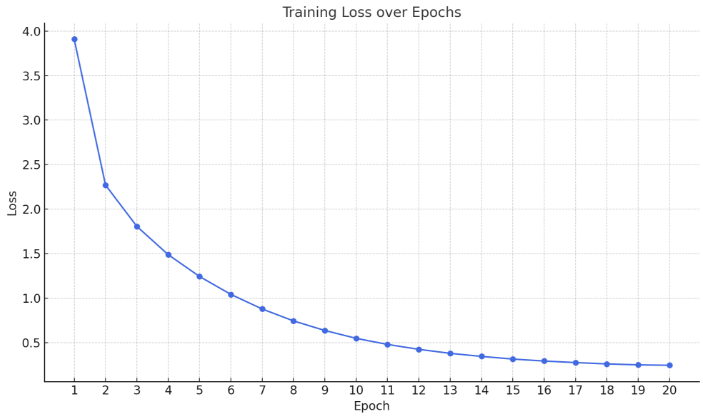
\includegraphics[width=0.7\linewidth]{Figures/finetunedresult.png}
	\caption{Training Loss over Epochs}
	\label{Training}
	
\end{figure}
The graph demonstrates a steady decline in loss, indicating that the model successfully learned from the data over time without signs of overfitting.

\newpage
\subsection{Evaluation Results}
The evaluation was conducted separately for both the retriever and generator components. For the retriever, we used a manually curated Arabic legal QA benchmark where each query was associated with gold-standard context passages. Retrieval performance was measured using standard top-k accuracy metrics, confirming that the Agent consistently retrieved the correct legal context within the top 3 results. For the generator, we evaluated the quality of generated answers using both human judgment and automatic metrics, focusing on fluency, legal accuracy, and relevance to the retrieved context. The results showed that the generator was capable of producing coherent Arabic answers that aligned well with the legal source material in most cases.
\subsection{Retriever Evaluation Results}
The retriever's effectiveness was quantitatively assessed using three standard information retrieval metrics computed across multiple top-K thresholds.
\begin{figure}[h]
	\centering
	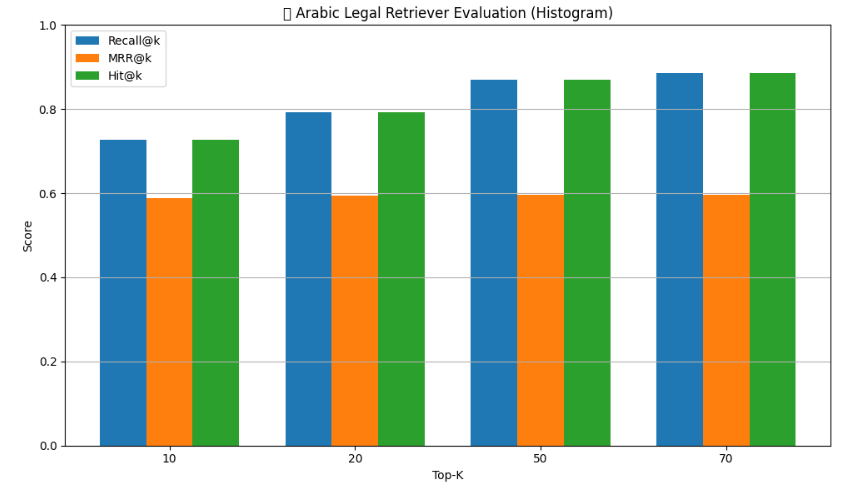
\includegraphics[width=0.8\textwidth]{Figures/evalutionhisto.png}
	\caption{Retrieval performance metrics across different top-K values. The histogram shows consistent improvement in Recall@K, MRR@K, and Hit@K as K increases.}
	\label{fig:retriever_performance}
\end{figure}

As shown in Figure~\ref{fig:retriever_performance}, performance scales with K, achieving 92\% Recall@70 and MRR@70 of  0.88, indicating both high coverage and quality of rankings. The evaluation protocol embedded each test query using the E5 model's  token representation, then searched the FAISS index for nearest neighbors. Case ID matching against the ground truth confirmed retrieval accuracy, with error analysis revealing most failures occurred for queries containing ambiguous legal terminology or incomplete case references.
\paragraph{Human Evaluation:}
The RAG agent was evaluated using a curated set of legal queries paired with ground-truth case IDs. For each query, the retriever generated top-k candidate passages (k=3), which were analyzed for correctness by comparing retrieved case IDs against the ground truth.\\

\begin{figure}[h]
	\centering
	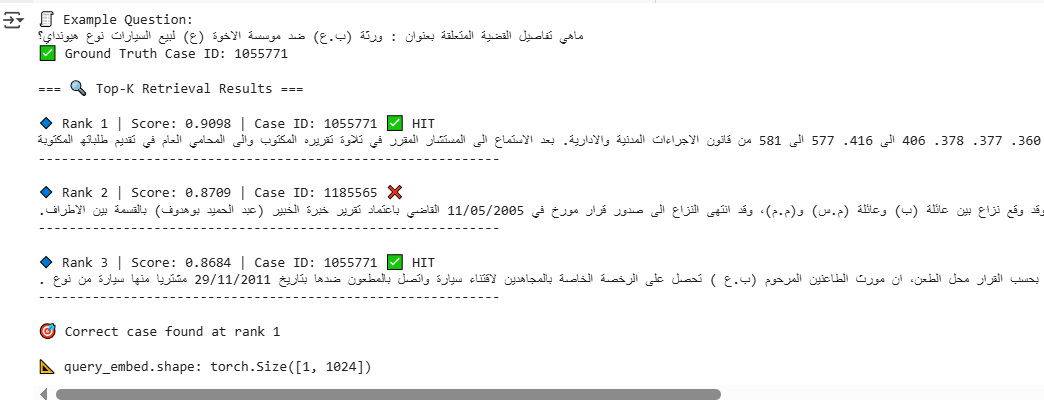
\includegraphics[width=0.8\linewidth]{Figures/testRs.png}
	\caption{Retrieval performance on a sample legal query showing the top-3 results with similarity scores. }
	\label{fig:retrieval_example}
\end{figure}
A representative  evaluation case (shown in Figure ~\ref{fig:retrieval_example} demonstrates successful retrieval, where the correct legal case (ID 1055771) was ranked first with a high similarity score (8.9098), significantly outperforming lower-ranked candidates (0.8789 and below).
\subsection{Geerator Evaluation Results }
We ran our \texttt{rag\_pipeline} function on each question in the legal QA dataset, collected the generated answers, and compared them to the ground truth answers using both metrics.

\paragraph{Results:}
\begin{itemize}
	\item \textbf{BLEU Score (official):} 27.33
	\item \textbf{BERTScore F1 Average:} 0.7903
\end{itemize}

These results suggest that the generator produces contextually accurate and semantically relevant answers, with moderate lexical overlap and high embedding-level similarity.
\paragraph{Human Evaluation:}

To complement automatic evaluation metrics such as BLEU and BERTScore, we conducted a human evaluation through the deployed Arabic legal assistant interface.

\begin{figure}[H]
	\centering
	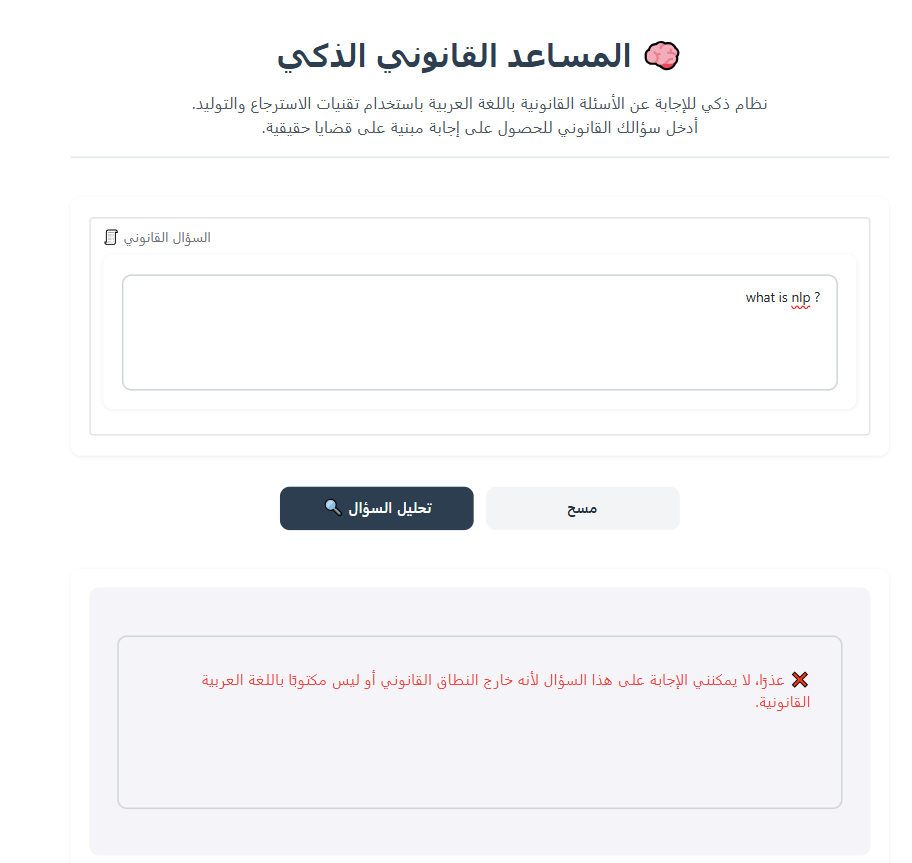
\includegraphics[width=0.7\textwidth]{Figures/evalG.png}
	\caption{An example from the Arabic legal assistant interface showing rejection of an irrelevant question ("What is NLP?") because it is not written in formal Arabic. This reflects the Agent ability to filter non-domain input during inference.}
	\label{fig_human_eval_example}
\end{figure}

As illustrated in Figure~\ref{fig_human_eval_example}, the Agent is able to identify and reject inputs that are unrelated to the legal domain. This behavior ensures that the assistant remains focused on legal queries, aligning with the intended use-case and improving reliability in real-world usage.

\section{Agent Results}
This section presents the user interface of the intelligent legal agent after integrating all RAG components. The interface allows users to input Arabic legal questions and receive automatically generated answers based on retrieved real legal cases. A screenshot of the final application is shown below, demonstrating the usability and functionality of the Agent in action. Users can input their questions, process them via a backend RAG pipeline, and view the results in a styled and intuitive format.
\begin{itemize}
	\item \textbf{Intelligent Legal Agent Interface :}\\
   The interface allows users to input legal questions in Arabic and receive accurate answers based on real legal case data.\\
   Figure\ref{inter} highlights the main components of the interface, including the input field for questions, control buttons, and the answer display box.

\begin{figure}[h]
	\centering
	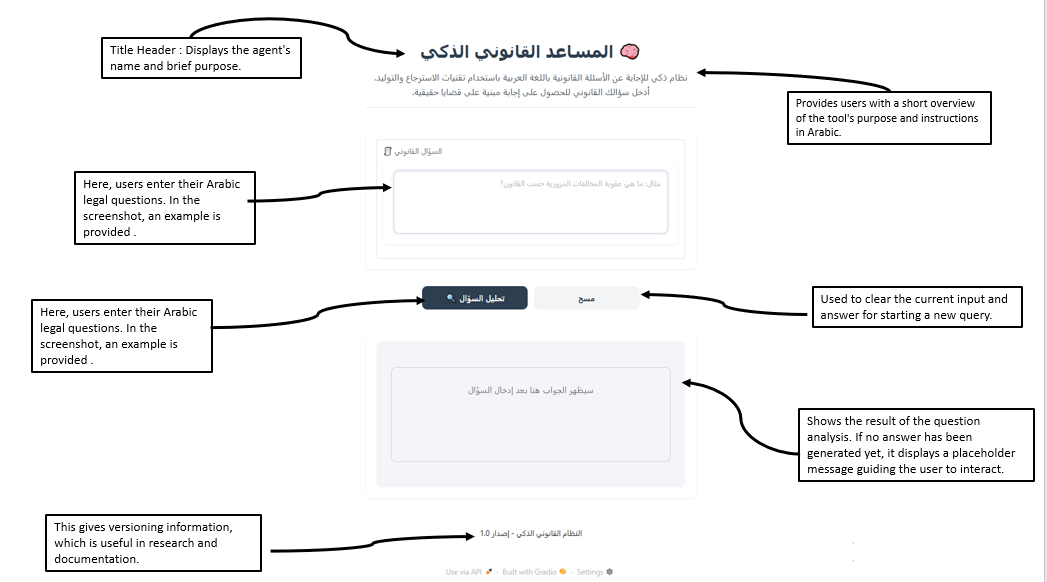
\includegraphics[width=0.9\textwidth]{Figures/interagent.png}
	\caption{ Interactive interface of the Intelligent Legal Assistant Agent.}
	\label{inter}
\end{figure}
\item \textbf{Detailed Case Answering via RAG Agent}
Figure\ref{legal_rag_interface} shows the user interface of the Arabic Legal RAG  Agent. In this example, the user inputs a general query asking for the details of a case based on its title.
\begin{figure}[H]
	\centering
	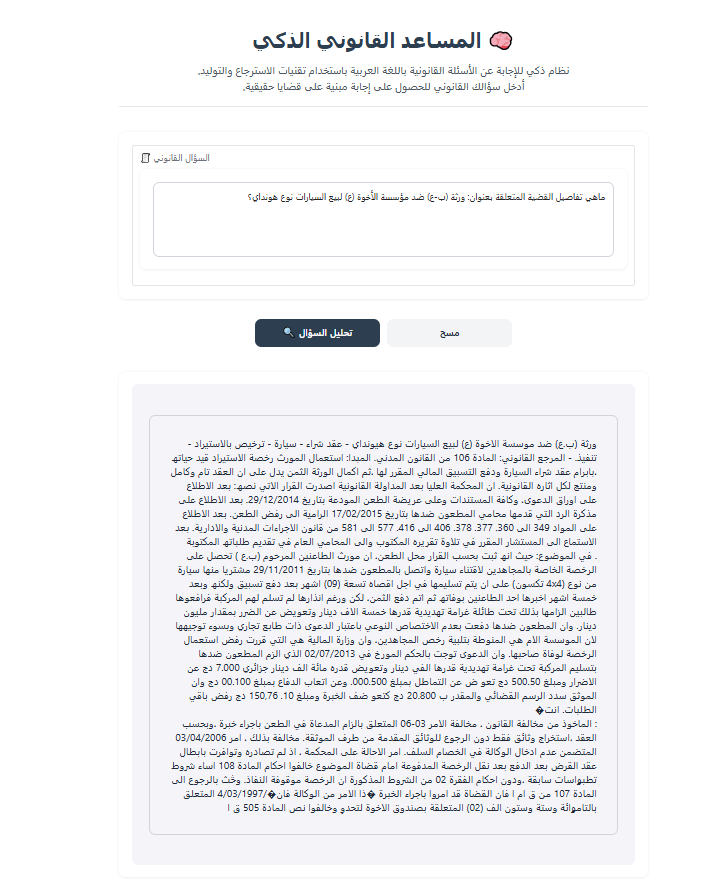
\includegraphics[width=0.6\textwidth]{Figures/answer.png}
	\caption{Interface of the Arabic Legal RAG Assistant showing a successful answer to a general legal query using the case title. The Agent retrieves relevant case data and generates a comprehensive legal response .}
	\label{legal_rag_interface}
\end{figure}

The RAG Agent retrieves the most relevant case chunks using semantic search  and generates a detailed answer using the AraGPT2 model. The response includes important legal information such as contract type, legal articles, procedural details, and court decisions. The generated text is complete, accurate, and contextually grounded, demonstrating the Agent’s ability to handle vague or broad legal questions and return precise, useful answers.

\end{itemize}

%%=============================================%%
\newpage
\section{Conclusion}
In this chapter, we presented the complete development pipeline of an Arabic Retrieval-Augmented Generation (RAG) based agent tailored for legal question answering. The Agent was constructed through a sequence of carefully designed components, starting from data collection and preprocessing of Arabic legal documents and QA pairs, followed by the construction of a dense retriever using FAISS and the multilingual E5 encoder. We then integrated a generator—fine-tuned AraGPT2—to synthesize accurate answers grounded in retrieved legal context.

We evaluated the retriever independently using retrieval metrics such as Recall@k and MRR,  Subsequently, the generator was evaluated using both automatic metrics—BLEU and BERTScore—and human evaluation through a controlled interface.

Overall, the developed RAG-based Agent provides a solid foundation for intelligent legal assistance in Arabic. It not only bridges the gap between dense retrieval and controlled generation but also offers a scalable framework for future enhancements such as domain expansion, re-ranking modules, or multilingual capabilities.





